\documentclass[12pt,letterpaper]{article}


\newcommand{\studentname}{Ben Bassett}
% \newcommand{\labpartner}{Katrina Sumarli}

\title{\textsc{Lab 05: An Application of Faraday’s Law}}
\newcommand{\shorttitle}{An Application of Faraday’s Law}

\newcommand{\course}{PHY310}
\newcommand{\labdate}{10-8-2024}

%------------------------------------------------------------------------------------------------------------

\usepackage[letterpaper,left=1in,right=1in,bottom=1in,top=1in]{geometry}
\usepackage{fancyhdr}
\usepackage{subfigure}
\usepackage{graphicx}
\usepackage{amsmath}
\usepackage{cleveref}
\usepackage{booktabs}
\usepackage[british]{babel}
\usepackage[square,comma,numbers,sort&compress]{natbib}
\usepackage{csvsimple}
\usepackage{graphicx}
\usepackage{pgfplotstable}
\usepackage{textcomp,gensymb}
\usepackage{array}
\usepackage{tabu}
\usepackage{multirow}
\usepackage{url}
\usepackage{lipsum}
\usepackage{dsfont}
\pgfplotsset{compat=1.9}% supress warning
\begin{document}

%------------------------------------------------------------------------------------------------------------

\setlength{\parindent}{1em}
\setlength{\parskip}{0.5em}
\author{\course~Lab Journal \\ \\ \studentname} % \,\& \labpartner}
\date{\labdate}

\renewcommand\abstractname{Summary}

\pagestyle{fancy}
\fancyhead{}
\fancyhead[l]{\course:~\shorttitle}
\fancyhead[r]{\studentname}
\fancyfoot{}
\fancyfoot[C]{\thepage}
\renewcommand{\headrulewidth}{0pt}
\renewcommand{\footrulewidth}{0pt}

\renewcommand\bibname{References}

%------------------------------------------------------------------------------------------------------------

\renewcommand\abstractname{Abstract}
\maketitle

% COMMENT IN IF ASKED TO SUBMIT REPORT WITH ABSTRACT
%\begin{abstract}
%Maximum 200 words.
%\end{abstract}

\section{Purpose}
This lab aimed to calculate the number of turns in a solenoid using Faraday’s Law.

\section{Experimental Apparatus}

Materials given were a Helmholtz Coil, function generator, DC power supply, magnetometer, instrumentation amplifier, ammeter, differential voltage probe, retort stand with clamp, solenoid, various cables, and a multimeter. My general setup is illustrated in Figure \ref{fig:setup}.

\begin{figure}[h]
    \centering
    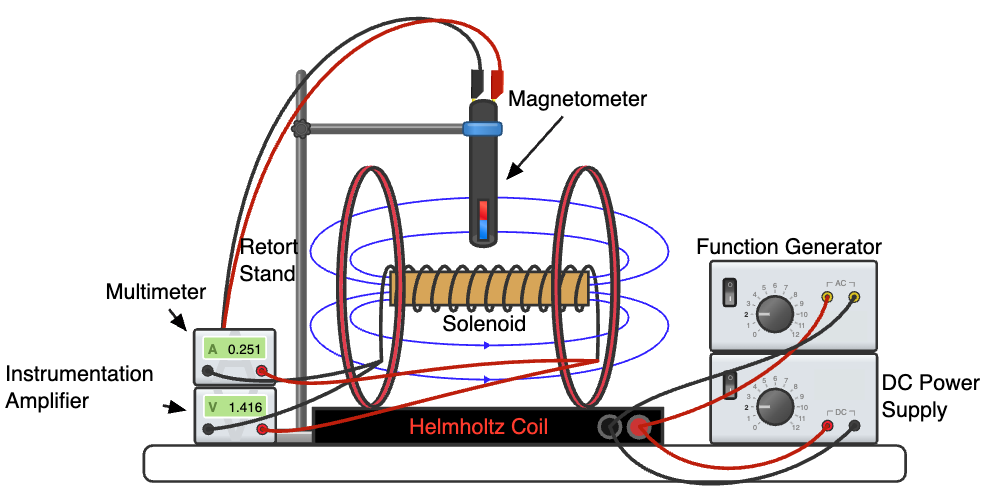
\includegraphics[width=6in]{images/setup.png}
    \caption{A diagram of my experimental setup}
    \label{fig:setup}
\end{figure}

% \pagebreak
\section{Procedure}

To begin, we needed to find the constant of linearity between current and B-field within the Helmholtz coil. To do so, we strapped the magnetometer onto the retort stand and suspended it in the middle of the Helmholtz coin, and used the DC power supply to record the magnetic field ever 0.5 amps from 0 to 3. 

Next, we needed to find where the current-voltage relationship within the coil obeyed Ohm's law. To do so, we attached the function generator to the Helmholtz coil and measured the current and voltage across the coils every 10 Hz from 0 to 300. However, we realized that this was insufficient, and so used the ammeter and differential voltage probe to measure those parameter from 1 to 10 Hz AC.

After we found where the Ohmic relationship held, we measured the EMF induced in the solenoid by suspending it in the Helmholtz coil with the retort clamp by attaching the instrumentation amplifier on the ±20 mV setting to the solenoid's connections.

\section{Results}

We measured the magnetic field within the coil every 0.5 amps from 0 to 3. Thankfully this was a perfectly linear relationship, which is represented in Figure \ref{fig:field}. We found this constant of linearity to be 0.8688.

\begin{figure}[ht]
    \centering
    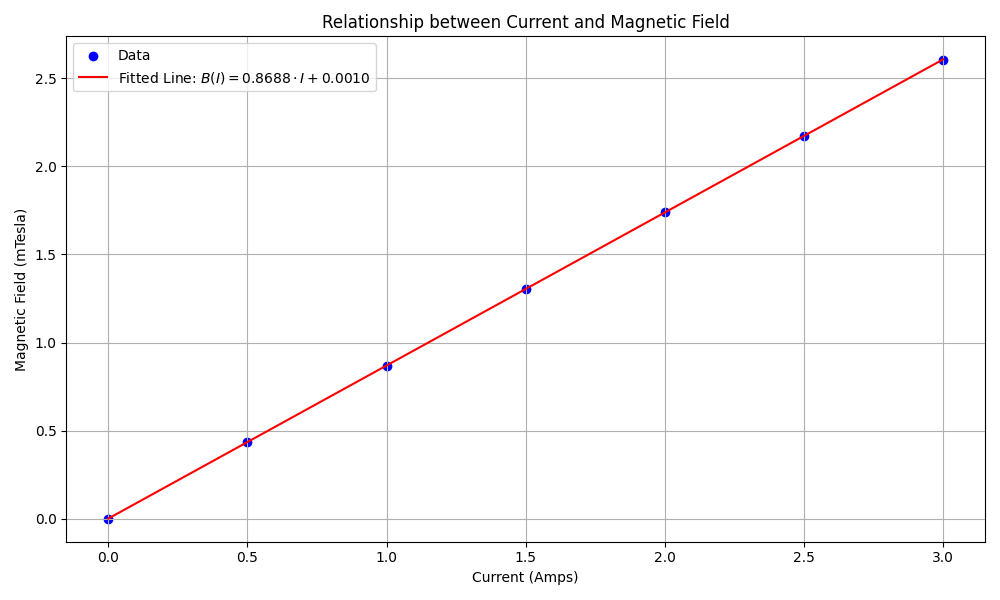
\includegraphics[width=5in]{images/Current_vs_Magnetic_Field.png}
    \caption{Current plotted against magnetic field}
    \label{fig:field}
\end{figure}

After this, we measured the resistance of our Helmholtz coil to be 3.8 $\Omega$. To see where the coil acted Ohmic, we measured voltage and current from 1 to 300 Hz in 10 Hz increments with the function generator set to 2 Hz. Looking through this data, we found found 20 Hz and above to give excessive resistance using Ohm's Law $R=\frac{V}{I}$. We went back and took the data again in a more granular fashion, and found 1 to 9 Hz to be the range within ± 0.1 $\Omega$ of the actual resistance. See this data in Table \ref{tab:ohmic}, with our errors propagated.

\begin{table}[ht]
\centering
\begin{tabular}{|l|l|l|l|}
\hline
 & Peak Voltage (V) & Peak Current (A) & Resistance ($\Omega$) \\ \hline
1 Hz & 1.8410 ± 0.0010 & 0.4871 ± 0.0010 & 3.7795 ± 0.0080 \\ \hline
2 Hz & 1.8410 ± 0.0010 & 0.4867 ± 0.0010 & 3.7795 ± 0.0080 \\ \hline
3 Hz & 1.8410 ± 0.0010 & 0.4837 ± 0.0010 & 3.7795 ± 0.0081 \\ \hline
4 Hz & 1.8524 ± 0.0010 & 0.4745 ± 0.0010 & 3.8030 ± 0.0083 \\ \hline
5 Hz & 1.8717 ± 0.0010 & 0.4447 ± 0.0010 & 3.8425 ± 0.0089 \\ \hline
6 Hz & 1.8869 ± 0.0010 & 0.4215 ± 0.0010 & 3.8738 ± 0.0094 \\ \hline
7 Hz & 1.8946 ± 0.0010 & 0.4131 ± 0.0010 & 3.8895 ± 0.0096 \\ \hline
8 Hz & 1.8946 ± 0.0010 & 0.3559 ± 0.0010 & 3.8895 ± 0.0111 \\ \hline
9 Hz & 1.8984 ± 0.0010 & 0.4284 ± 0.0010 & 3.8973 ± 0.0093 \\ \hline
\end{tabular}
\caption{Peak values of frequency, voltage, current, and resistance}
\label{tab:ohmic}
\end{table}

Having found the working range for the coil, we measured peak EMF from the instrumentation amplifier from 1 to 9 Hz in Table \ref{tab:turns}. To apply this data, Let's derive the equation for the number of turns ($n$) in a solenoid from Faraday's Law:

\begin{align*}
    \oint \vec{E}\cdot d\vec{l}&=-\frac{d\Phi_B}{dt}=\varepsilon \\
    \varepsilon(t)&=n\pi r^2 \frac{dB}{dt}c \text{ (constant of linearity)} \\
    B(t)&=I_0e^{i2\pi ft} \\
    \varepsilon(t)&=\varepsilon_0e^{i2\pi f t} \\
    n&= \frac{\varepsilon(t)}{\pi r^2 \frac{dB}{dt}c} \\
    \text{Re}\left\{\frac{dB}{dt}\right\}&=I_02\pi f\cos\left(2\pi f  - \frac{\pi}{2}\right) \\
    n&=\frac{\varepsilon_0\cos(2\pi fa)}{2\pi^2 r^2 I_0 \cos\left(2\pi f - \frac{\pi}{2}\right)f c} \text{ (ignore phase offsets)}\\
    n&=\frac{\varepsilon_0}{2\pi^2 r^2 I_0 f c}
\end{align*}

I used the final expression to compute all the turns using the measured peak EMF, current, and frequency, as well as 0.8688 as our constant of linearity and 22 mm as the diameter of our solenoid. See my results with propagated error in Table \ref{tab:turns}.

\begin{table}[ht]
\centering
\begin{tabular}{|l|l|l|l|}
\hline
  & Peak EMF (mV) & Peak Current (A) & Number of Turns ($n$) \\ \hline
1 Hz & 64.8023 ± 0.0010 & 0.4871 ± 0.0010 & 1604.2754 ± 3.2936 \\ \hline
2 Hz & 102.4546 ± 0.0010 & 0.4867 ± 0.0010 & 1269.1993 ± 2.6077 \\ \hline
3 Hz & 151.8805 ± 0.0010 & 0.4837 ± 0.0010 & 1262.2368 ± 2.6097 \\ \hline
4 Hz & 201.3064 ± 0.0010 & 0.4745 ± 0.0010 & 1279.0122 ± 2.6956 \\ \hline
5 Hz & 243.6681 ± 0.0010 & 0.4447 ± 0.0010 & 1321.3903 ± 2.9712 \\ \hline
6 Hz & 269.5467 ± 0.0010 & 0.4215 ± 0.0010 & 1285.3010 ± 3.0495 \\ \hline
7 Hz & 308.4940 ± 0.0010 & 0.4131 ± 0.0010 & 1286.5465 ± 3.1146 \\ \hline
8 Hz & 302.0420 ± 0.0010 & 0.3559 ± 0.0010 & 1279.2756 ± 3.5946 \\ \hline
9 Hz & 407.3458 ± 0.0010 & 0.4284 ± 0.0010 & 1274.1624 ± 2.9746 \\ \hline
\end{tabular}
\caption{Peak values of frequency, EMF, current, and number of turns}
\label{tab:turns}
\end{table}

Finally, we were asked to plot the relationship between peak EMF and the frequency of voltage, which is visible in Figure \ref{fig:emf} with a linear fit that has an R$^2$ of 0.9692.

\begin{figure}[ht]
    \centering
    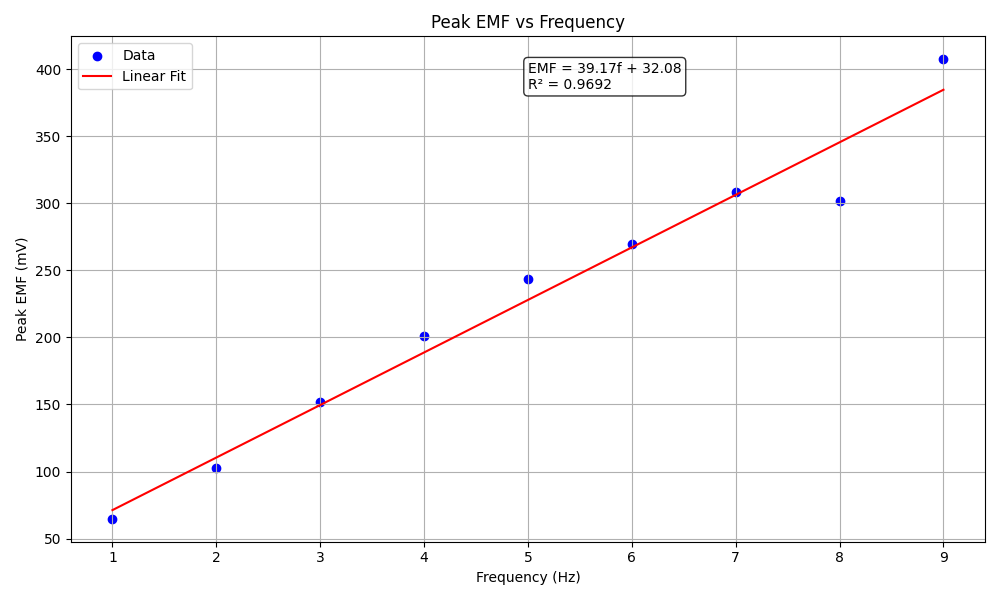
\includegraphics[width=5in]{images/peak_emf_vs_frequency_fit.png}
    \caption{Peak EMF $\varepsilon$ plotted against voltage frequency}
    \label{fig:emf}
\end{figure}

I used this fit to compute the number of turns by taking an average of all the computed values for solenoid turns over the 1-9 Hz range. This gives us a final answer of $\mathbf{1317.9333 \pm 3.0060} \textbf{ turns}$.

\section{Conclusions}

While the actual solenoid does not seem to have that many turns to my eye, our process was rigorous and sound in theory. Our greatest source of error was likely our resistance, as we measured it once at the beginning of the experiment, then collected the rest of our data. But trying to re-evaluate our processes we measured it again and it appeared significantly higher. I used the original value for analysis since it was what we consistently worked with when first gathering data. Moving the coil or switching multimeters or cables slightly seemed to change the value. In addition, the instrumentation amplifier seems like a weak link in the data collection process as it seems to artificially inflate or deflate the actually EMF depending on where the amplification dial is set. So while our analysis is sound, the experimental processes could do with some improvement.


% \bibliographystyle{unsrtnat}
% \bibliography{references}

\end{document}
